\documentclass[crop,tikz]{standalone}

\usepackage[utf8]{inputenc}

% 'crop' is the default for v1.0, before it was 'preview'
%\usetikzlibrary{...}% tikz package already loaded by 'tikz' option

\begin{document}

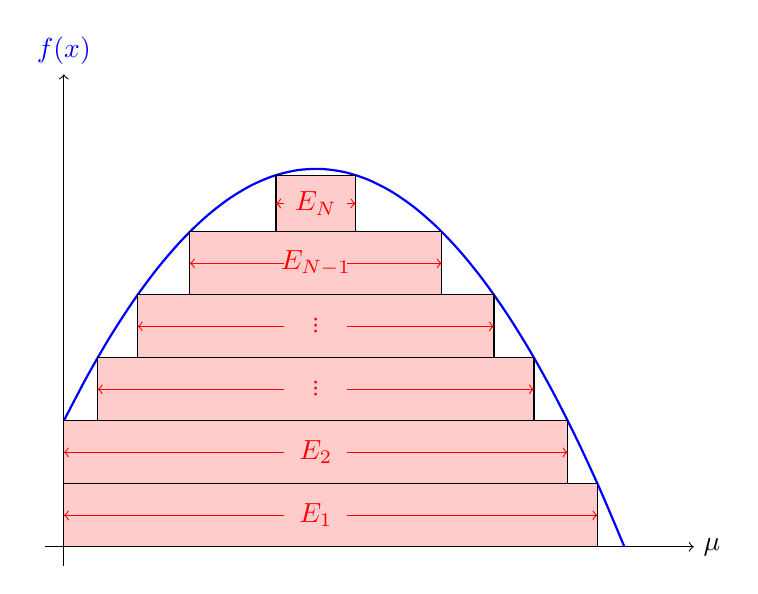
\begin{tikzpicture}

	\begin{scope}[scale=0.8]
		\draw[->] (-0.3,0) -- (10,0) node[anchor=west] {$\mu$};
		\draw[->] (0,-0.3) -- (0,7.5);
		\node[anchor=south, color=blue] at (0,7.5) {$f(x)$};
		\draw[scale=1.0,domain={0:8.89897},smooth,variable=\x,blue, thick] plot ({\x}, {(-(0.5*\x-2)*(0.5*\x-2)+6});
		
		%division of the range
		\draw[black, fill=red!20!white] (0,0) rectangle (8.4721,1);
		\draw[black, fill=red!20!white] (0,1) rectangle (8,2);
		\draw[black, fill=red!20!white] (0.5359,2) rectangle (7.4641,3);
		\draw[black, fill=red!20!white] (1.1716,3) rectangle (6.8284,4);
		\draw[black, fill=red!20!white] (2,4) rectangle (6,5);
		\draw[black, fill=red!20!white] (3.36754,5) rectangle (4.63246,5.9);

		%box labels
		\draw[->, red] (4-0.5,0.5) -- (0,0.5); 
		\draw[->, red] (4+0.5,0.5) -- (8.4721,0.5);
		\node[align=center, red] at (4,0.5) {$E_1$};
		\draw[->, red] (4-0.5,1.5) -- (0,1.5); 
		\draw[->, red] (4+0.5,1.5) -- (8,1.5);
		\node[align=center, red] at (4,1.5) {$E_2$};
		\draw[->, red] (4-0.5,2.5) -- (0.5359,2.5); 
		\draw[->, red] (4+0.5,2.5) -- (7.4641,2.5);
		\node[align=center, red] at (4,2.6) {$\cdot$};
		\node[align=center, red] at (4,2.5) {$\cdot$};
		\node[align=center, red] at (4,2.4) {$\cdot$};
		\draw[->, red] (4-0.5,3.5) -- (1.1716,3.5); 
		\draw[->, red] (4+0.5,3.5) -- (6.8284,3.5);
		\node[align=center, red] at (4,3.6) {$\cdot$};
		\node[align=center, red] at (4,3.5) {$\cdot$};
		\node[align=center, red] at (4,3.4) {$\cdot$};
		\draw[->, red] (4-0.5,4.5) -- (2,4.5); 
		\draw[->, red] (4+0.5,4.5) -- (6,4.5);
		\node[align=center, red] at (4,4.5) {$E_{N-1}$};
		\draw[->, red] (4-0.5,5.45) -- (3.36754,5.45); 
		\draw[->, red] (4+0.5,5.45) -- (4.63246,5.45);
		\node[align=center, red] at (4,5.45) {$E_{N}$};
	\end{scope}

\end{tikzpicture}

\end{document}